\documentclass[../TST.tex]{subfiles}
\begin{document}
\begin{pproblem}[Alloy density]
Gold-copper alloys $\mathrm{Au}_x\mathrm{Cu}_{1-x}$ (of number fraction $x$) have a face-centred cubic lattice, as shown on Figure \ref{fig2}. The atoms of copper and gold are randomly distributed on the lattice points. The density of pure gold is $\rho_\mathrm{Au}=\qty{19.30}{g/cm^3}$, its lattice constant is $a_\mathrm{Au}=\qty{4.078}{\angstrom}$ , while the density of pure copper is $\rho_\mathrm{Cu}=\qty{8.96}{g/cm^3}$ and its lattice constant is $a_\mathrm{Cu}=\qty{3.615}{\angstrom}$. Assume that the lattice constant is proportional to $x$. Let $y$ be the mass fraction of the alloys $\mathrm{Au}_x\mathrm{Cu}_{1-x}$, such that $y=\frac{m_\mathrm{Au}}{m_\mathrm{Cu}+m_\mathrm{Au}}$.
\begin{enumerate}
	\item Find the number fraction in terms of the mass fraction, $x=f(y)$.\score{1.0}
	\item Find the density in terms of the mass fraction, $\rho_{\mathrm{Au}_x\mathrm{Cu}_{1-x}}=f(y)$.\score{1.0}
	\item Find the density of a gold-copper alloy for mass fractions $y=0.5$ and $y=0.8$.\score{1.0}
\end{enumerate}
\begin{figure}[h]
\centering
\hspace*{1ex}
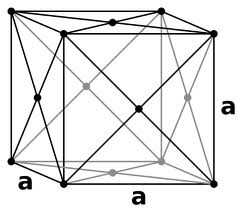
\includegraphics[width=0.3\textwidth]{fig/2015_l4.jpg}
\caption{}
\label{fig2}
\end{figure}
\end{pproblem}

\ifprob \else
	\begin{solution} (a) Each unit cell is a cube of side $a$. Within the cell, there are 8 atoms at the vertices which are shared between 8 cubes each, and there are 6 atoms at the faces which are shared between 2 cubes each. In total there are $8\cdot \frac{1}{8}+ 6\cdot \frac{1}{2}=4$ atoms per unit cell. This means that $\rho_\mathrm{Au}a_\mathrm{Au}^3=4M_\mathrm{Au}$ and $\rho_\mathrm{Cu}a_\mathrm{Cu}^3=4M_\mathrm{Cu}$, where $M_\mathrm{Au}$ and $M_\mathrm{Cu}$ are the masses of a single gold or copper atom. \\[5pt]
		The mass fraction can be found by comparing the total masses of each element:
		\begin{equation*}
		y=\frac{m_\mathrm{Au}}{m_\mathrm{Cu}+m_\mathrm{Au}}= \frac{M_\mathrm{Au}x}{M_\mathrm{Au}x+M_\mathrm{Cu}(1-x)}
		.
		\end{equation*}
We rearrange this to get $x$ in terms of $y$:
\begin{equation*}
	x=\frac{M_\mathrm{Cu}y}{M_\mathrm{Cu}y+M_\mathrm{Au}(1-y)}=\frac{y}{y+\frac{M_\mathrm{Au}}{M_\mathrm{Cu}}(1-y)}=\boxed{\frac{y}{y+\left(\frac{\rho_\mathrm{Au}a_\mathrm{Au}^3}{\rho_\mathrm{Cu}a_\mathrm{Cu}^3}\right) (1-y)}.}
\end{equation*}
(b) The lattice constant $a$ is proportional to $x$, and we know that $a=a_\mathrm{Cu}$ at $x=0$ (no gold) and $a=a_\mathrm{Au}$ at $x=1$ (no copper). The formula for $a$ in terms of $x$ should then be
\begin{equation*}
a=a_\mathrm{Cu}+(a_\mathrm{Au}-a_\mathrm{Cu})x
.
\end{equation*}
The density can be found as the mass of the atoms in a cell, divided by the volume of a cell.  The total mass of the atoms is equal to that of just the gold atoms, divided by $y$:
\begin{equation*}
\rho = \frac{M_\mathrm{cell}}{a^3}= \frac{M_\mathrm{cell}(\mathrm{Au})}{a^3}\left(\frac{1}{y}\right) 
.
\end{equation*}
As discussed above, 4 sites with gold atoms would have a total mass of $\rho_\mathrm{Au}a_\mathrm{Au}^3$. However, only a fraction $x$ of the sites are actually occupied by gold atoms, so
\begin{equation*}
	\rho = \frac{\rho_\mathrm{Au}a_\mathrm{Au}^3}{a^3}\left(\frac{x}{y}\right)  =\frac{\rho_\mathrm{Au}a_\mathrm{Au}^3}{(a_\mathrm{Cu}+(a_\mathrm{Au}-a_\mathrm{Cu})x)^3}\left(\frac{x}{y} \right) =\rho_\mathrm{Au}\left(\frac{a_\mathrm{Cu}}{a_\mathrm{Au}}+ \left(1-\frac{a_\mathrm{Cu}}{a_\mathrm{Au}}\right)x \right)^{-3}\left(\frac{x}{y} \right).
\end{equation*}
We're still not done, because the expression should be in terms of $y$ only. Using our result in (a), we can reach
\begin{equation*}
\boxed{	\rho=\rho_\mathrm{Au}\left(y+\left(\frac{\rho_\mathrm{Au}a_\mathrm{Au}^3}{\rho_\mathrm{Cu}a_\mathrm{Cu}^3}\right) (1-y)\right)^{-1}\left(\frac{a_\mathrm{Cu}}{a_\mathrm{Au}}+ \left(1-\frac{a_\mathrm{Cu}}{a_\mathrm{Au}}\right)\left(1+\frac{\rho_\mathrm{Au}a_\mathrm{Au}^3}{\rho_\mathrm{Cu}a_\mathrm{Cu}^3}\cdot \frac{1-y}{y}\right)^{-1}  \right)^{-3}
.}
\end{equation*}
This is awful, and it is essential to do a safety check. The expression should reduce to $\rho_\mathrm{Cu}$ for $y=0$ and $\rho_\mathrm{Au}$ for $y=1$. And indeed, it does.\\

(c) To prepare for the calculation, you should first write down $\frac{a_\mathrm{Cu}}{a_\mathrm{Au}}=0.887$ and $\frac{\rho_\mathrm{Au}a_\mathrm{Au}^3}{\rho_\mathrm{Cu}a_\mathrm{Cu}^3}=3.092$. It is safer to compute this in chunks rather than in one go. Commit the intermediate values to paper in case you slip up with the calculator. The answers for $y=0.5$ and $y=0.8$ are $\boxed{\rho=\qty{12.34}{g/cm^3}}$ and $\boxed{\rho=\qty{15.84}{g/cm^3}}$, respectively.



\end{solution}
\fi
\end{document}
